\section{Active Galactic Nuclei}
\subsection{The Physical Nature of AGN Emissions}
An active galaxy hosts an AGN component in the central nucleus. One of the first discovered active galaxies was by Carl Seyfert in 1943 \citep{seyfert_nuclear_1943}. The Seyfert galaxies referred to a particular type of galaxy that hosted broad emission lines, an extremely luminous galactic nucleus and a visible host galaxy. A second class of active galaxy was later identified by \cite{schmidt_3c_1963}, originally thought to be star-like objects at high redshifts. These star-like objects were referred to as quasi-stellar objects (QSO) or quasars, and it was later confirmed by \cite{salpeter_accretion_1964} and others to be supermassive black holes accreting large amounts of matter with intense luminosity outshining its host galaxy. While it was not entirely clear then, it was eventually discovered that these two interstellar objects were related, with quasars hosting an AGN with sufficient luminosity to outshine their host galaxy, unlike the lower-luminosity Seyfert galaxies. The different classes of active galaxies have since been rigorously studied, leading to an 'AGN Zoo' of classes \citep{padovani_active_2017}. While many types of active galaxies are being studied, the physical nature of the AGN is still a heavily debated topic, and various schools of thought exist on the formation of AGN, its physical structure, and its relation to its host galaxy. Although the supermassive black hole is confirmed to drive the accretion of matter, many other physical components are still being studied today. Most AGN are thought to contain the following: the central black hole, a surrounding accretion disk, high-density dust-free gas clouds, a torus of dust, lower-density ionised gas, and, depending on the AGN type, a central jet of ionised matter \citep{netzer_revisiting_2015}. A simplified model of an AGN showing its physical components is shown in Figure \ref{fig:agn_schematic}.\\
\begin{figure}[h!]
    \centering
    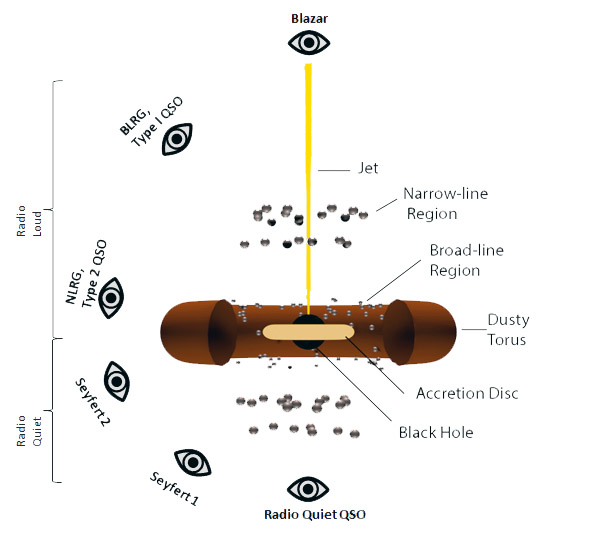
\includegraphics[width=1\textwidth]{Images/TheoreticalModelPlots/AGN_Thesis_Diagram_white.jpg}
    \caption{Schematic diagram of an AGN (adapted from  \citealt{urry_unified_1995}) showing most of the physical components. Also shown is the field of view that determines the classification type.}
    \label{fig:agn_schematic}
\end{figure}
In the region outside of the black hole lies a large disc of gas and dust undergoing the accretion process. This accretion disc model was proposed as an explanation for the extreme luminosity and emission line spectra of active galaxies, and there have been a variety of proposals of different accretion disk models for different AGN types \citep{netzer_revisiting_2015}. \cite{narayan_advection-dominated_1995} and \cite{esin_hot_1996} suggested an optically thin and geometrically thick disk, while \cite{shakura_black_1973} imagined an optically thick and geometrically thin disc of inflowing material. These two opposing viewpoints on the physical structure of the accretion disk were later reconciled by subsequent research, with current theories proposing that the accretion rate influences the geometry and optical properties of the disc \citep{abramowicz_foundations_2013}. While it is still a topic of research, it is highly suggested in the literature that above the disc, there is a hot structure known as the accretion disc corona, whereby gravitational power is dissipated, and magnetic fields reconnect, similar in principle to the sun's corona \citep{haardt_two-phase_1991}. Further out from the accretion disc, two separate regions are thought to be responsible for the broad and narrow line spectrum observed in AGN candidates. The first of these two regions, and the region responsible for the broadlines, is aptly named broad line region (BLR). This region is thought to consist of high-density dust-free gas clouds ($\approx 10^{11}$ cm$^{-3}$) stretching from 0.01 to 1 parsec (pc) from the central black hole \citep{baskin_dust_2018}. The broad lines observed in the spectrum of a BLR result from Doppler broadening, whereby a distribution of velocities of ionised molecules is observed due to the Doppler effect. Due to our distance from this region and its comparatively small size, this region was previously unable to be spatially resolved. However, recent observations with the GRAVITY instrument \citep{eisenhauer_gravity_2011} on the Very Large Telescope Interferometer (VLTI) allowed sub-parsec spatial resolution of the rotation of BLR \citep{gravity_collaboration_spatially_2018}, with additional follow up studies by the GRAVITY collaboration spatially resolving the BLR  \citep{gravity_collaboration_spatially_2020}. Looking beyond the BLR, we find a narrow line region (NLR) of ionised gas and dust responsible for the narrow line emission observed in various AGN sources. The narrow lines occur due to gas ionisation occurring further from the SMBH, causing strong narrow peaks unaffected by Doppler broadening. While the exact origin of the NLR is unclear, the size ($\sim10^{2}-10^{4}$pc) of this region allows for studies into its kinematics and morphology due to its being able spatially resolved \citep{joh_gas_2021}. The dusty torus is located between the narrow-line and broad-line regions and is an axisymmetric dusty structure on the scale of around 0.1-10 pc \citep{netzer_revisiting_2015}. This structure is known to be both geometrically and optically thick and has the potential to obscure both the broad-line region and the accretion disc. The nature and composition of this structure are still heavily researched, with different models that attempt to recreate the emission characteristics. In particular, \cite{fritz_revisiting_2006} proposed a toroidal, flared structure with a distribution of grain types; in this model, Fritz argued that `the dusty torus could be represented by a smooth distribution of dust particles in a sort of two-phase dust distribution around the accretion disc'. Later work by \cite{stalevski_3d_2012} imagined the structure with a similar two-phase toroidal geometry, and instead of a smooth dust distribution, they envisioned the dusty torus as clumpy and inhomogeneous. While there is no consensus on which model is correct, mounting evidence supports a clumpy two-phase dusty torus \citep{nikutta_hypercubes_2021}. Finally, some AGN produce powerful relativistic jets that extend far beyond their host galaxy into the surrounding intergalactic environment. These jets were first categorised by \cite{fanaroff_morphology_1974} as radio jets with distinct morphologies and are thought to be produced above the SMBH as a collimated outflow of particles \citep{blandford_relativistic_2019}. It is still not fully understood why some AGN have jets present while others do not; it is thought, however, that this process is largely driven by the dissipation of rotational energy from a black hole through the Blandford-Znajek process \citep{blandford_electromagnetic_1977}. Each physical component of an AGN is responsible for the emission across different wavelengths, with dominant emission processes responsible for each wavelength (see Table \ref{tab:agn_emission}). Optical and UV emissions are attributed to the accretion disk and the BLR \citep{czerny_origin_2011}. The most accepted theory of x-ray emission is due to inverse Compton scattering, wherein lower energy photons are boosted to higher energies through electron collisions \citep{haardt_two-phase_1991, padovani_active_2017}. Outside of the accretion disk, due to the obscuring torus, optical, UV and X-ray light is reprocessed by the torus's dust, which is anisotropically re-emitted in the infrared (IR; \citealt{stern_midinfrared_2005}). The powerful relativistic jets are thought to be responsible for radio and gamma-ray production \citep{hardee_agn_2008}. 
\begin{table}[h!]
    \centering
    \begin{tabular}{llp{4.5cm}}  % Adjust the width (4cm) as needed for your document
        \hline
        \textbf{Band} & \textbf{Primary Emission Region} & \textbf{Physical Process} \\ \hline
        Radio & Jets & Synchrotron radiation \\
        Infrared & Dusty Torus & Thermal emission from dust grains \\
        Ultraviolet/Optical  & Accretion Disk & Thermal emission from hot gas \\
        X-ray & Corona, Jet Base & Inverse Compton scattering, thermal bremsstrahlung \\
        Gamma-ray & Jets & Inverse Compton scattering \\ 
        \hline
    \end{tabular}
    \caption{Electromagnetic emission in each wavelength band and their primary sources within an AGN based on the unified model. Note that some regions may contribute to multiple bands (Adapted from \citealt{padovani_active_2017})}
    \label{tab:agn_emission}
\end{table}
\subsection{Classification Schemes and Terminology}
Historically, different types of AGN were perceived as distinct, unrelated objects due to the variation in observed phenomena. This led to many classification schemes and nomenclature, which persisted well after discovering that these objects were manifestations of the same underlying phenomenon. An attempt to unite these disparate classes of AGN was realized in the form of the Unified Model of Active Galactic Nuclei (See Figure \ref{fig:agn_schematic}; \citealt{rowan-robinson_unity_1977, antonucci_unified_1993, urry_unified_1995}). While this unification scheme allowed AGN to be explained based on a few physical parameters, some of the nomenclature has persisted. Generally, AGN unification models are often divided into radio and non-radio unification schemes. For non-radio unification, AGN can be categorised into two broad classes delineated by their viewing angle to the central engine (See Figure \ref{fig:agn_schematic}). These are commonly called Type 1 and Type 2 AGN \citep{netzer_revisiting_2015}. AGN, where the engine is unobscured and directly observable, are categorised as Type 1 AGN. This unobstructed view allows for the clear detection of broad emission lines and some high-ionisation narrow lines \citep{antonucci_spectropolarimetry_1985}. Similarly, AGN with an obscured view of the central engine, and thus the broad line emitting region, are referred to as Type 2 AGN. Although the unified model, and by extension, Type 1 and Type 2 classifications, are supported within the literature, it is still regarded as an incomplete theory. The unified model assumes all AGN are intrinsically the same when, in reality, there is a diversity of different AGN types. \cite{elitzur_disc_2016} discusses an example of this in which some AGN lack broad emission lines and have little to no obscuration to the central source, thus not categorically fitting into either Type 1 or Type 2. As previously discussed, UV-optical light is mostly produced in the accretion disk and BLR; this results in Type 1 AGN appearing more blue in general, while Type 2 AGN appear redder due to the IR excess caused by the reprocessing of the UV-optical light by the obscuring dusty torus. The radio unification scheme similarly takes a simplified approach to the classification of AGN, which involves splitting AGN into two main classes: Radio-Loud AGN (RLAGN), which is characterised by luminous relativistic jet-driven radio emission, and the Radio-Quiet AGN (RQAGN) which produce energetically insignificant radio emission \citep{wilson_difference_1995}. While this nomenclature persists, efforts have been made to create a grand unified model scheme and to tidy up the nomenclature. In particular, \cite{padovani_two_2017} advocates for referring to the two main classes of AGN as jetted and non-jetted and for explaining all AGN types in terms of three parameters: the orientation, lack or presence of jets, and the accretion rate. 